\section{Vista de procesos}
\label{sec:vista-procesos}

\subsection{Particionado y aislamiento de ejecuciones}
\label{subsec:particionado-aislamiento}
Una partición, o \emph{shard}, es una porción del trabajo y de su estado.
Antes de iniciar cada ejecución se fija la cantidad de particiones por etapa
y se configura qué instancia de worker, alojada en qué contenedor, es
propietaria de cada una. Para las operaciones
por palabra se aplica una función hash estable:
\[
    p(w) = H(w) \bmod P,
\]
donde $w$ es la palabra y $P$ la cantidad de particiones de la etapa. La
configuración relaciona el identificador $p$ con el worker y su contenedor;
el hash no selecciona por sí solo una máquina. Por ejemplo, con cuatro
particiones, un worker puede atender las particiones 0 y 1, y otro las 2 y 3.
Los aportes de una misma palabra llegan a su propietario. El trabajo por
artículo se reparte por identidad del registro o por lotes de entrada.

Cada partición tiene un único propietario activo de sus acumuladores, archivos
y progreso. Un worker puede atender varias particiones; agrupar workers en
un contenedor no fusiona sus estados ni sus responsabilidades. Las cantidades y
asignaciones permanecen estables durante la ejecución; se redistribuyen antes
de nuevas ejecuciones. El manifiesto registra los participantes y destinos
esperados para verificar los cierres.

La identidad de ejecución forma parte de las claves de estado, los mensajes y
las rutas de archivos. Compartir un contenedor o una partición entre clientes
no mezcla sus datos. \texttt{TopKReducer}, \texttt{Average Calculator} y
\texttt{ResultCollector} tienen un propietario por ejecución, distribuido entre
las instancias disponibles; no existe un único propietario global para todos
los clientes. Q4 y Q5 sólo se entregan después de procesar todo el input;
Q1--Q3 pueden entregarse parcialmente con seguimiento de cierre.

\subsection{Gestión del estado y límites de recursos}
\label{subsec:estado-recursos}
Los archivos temporales pertenecen a los workers que necesitan conservar
estado y se ubican en montajes locales de sus hosts, separados por ejecución
y partición. Su uso depende del rol:
\begin{itemize}
    \item Q3: \texttt{WordAppearenceDetector} conserva presencia por idioma y
    seguimiento de palabras emitidas, con archivos cuando el vocabulario
    excede el presupuesto de memoria.
    \item Q4: \texttt{WordCountReducer} vuelca conteos parciales a disco y los
    combina para mantener memoria acotada ante vocabularios grandes.
    \item Q5: \texttt{Average Filter} guarda en disco los candidatos posteriores
    a 2020, al menos su URL y conteo de palabras, hasta recibir el promedio
    histórico definitivo. Luego recorre esos archivos y emite los que superan
    el umbral. Asume esta responsabilidad sin un nodo aparte. Lo mismo ocurre en \texttt{Average Calculator} mientras se esperan todos las longitudes requeridas para calcular el promedio.
    \item Q2: \texttt{ImageFetcher} guarda temporalmente las imágenes descargadas
    y las lee en fragmentos acotados para enviarlas por RabbitMQ a
    \texttt{ResultCollector}, luego a \texttt{Gateway} y finalmente al cliente.
    Estos archivos de trabajo no constituyen un snapshot
    persistente ni un servicio de archivos compartidos.
\end{itemize}
No todos los workers acceden a estos archivos: cada propietario administra
los suyos. No se introduce una base de datos ni un almacenamiento compartido
central del corpus. Q4 recibe su orden del \texttt{TopKReducer}; no se incorpora
una ordenación global de las otras salidas en \texttt{ResultCollector}.

Cada instancia limita memoria, lotes, entregas pendientes, descargas y disco
por ejecución. Frente a clientes lentos, Gateway y ResultCollector mantienen
buffers acotados. Las colas y publicaciones pendientes de RabbitMQ también
deben tener límites: no se sustituye el disco del collector por acumulación
ilimitada en el broker. El seguimiento de entrega y deduplicación debe liberar
estado confirmado sin crecer con toda la salida histórica.
Al agotarse una cuota se suspende la admisión o se informa cancelación o fallo.
Los archivos temporales se eliminan al completar la entrega o terminar el intento.

\subsection{Diagramas de actividades}
En esta sección se presentan algunos diagramas que ilustran cómo actuarán los nodos en conjunto.

\subsubsection{Consulta n°1}
Para la primer funcionalidad, mostramos como el nodo de \textit{Date Filter} elimina del pipeline aquellos datos coyo año sea mayor al 2020, y propaga el EOF sin una lógica adicional. Finalmente, el último filtro se queda únicamente con la data en inglés 
\begin{figure}[H]
    \centering
    \includesvg[width=\textwidth,height=0.82\textheight,keepaspectratio]{img/Act/query_1_Act.drawio}
    \caption{Url y fecha de modificación para artículos escritos en inglés hasta 2020 inclusive.}
    \label{fig:query-1}
\end{figure}


\subsubsection{Consulta n°2}
Siguiendo el flujo del DAG, no volvemos a repetir el nodo de \textit{Date Filter} para el diagrama de la siguiente consulta que sí forma parte del pipeline, pero para simplificar no lo agregamos.
\begin{figure}[H]
    \centering
    \includesvg[width=\textwidth,height=0.82\textheight,keepaspectratio]{img/Act/query_2_Act.drawio}
    \caption{Nombre, url e imágen (bytes) de artículos escritos hasta 2020 inclusive que incluyan
“biography” o “biographie” entre sus secciones.}
    \label{fig:query-2}
\end{figure}

\subsubsection{Consulta n°3}
\begin{figure}[H]
    \centering
    \includesvg[width=\textwidth,height=0.82\textheight,keepaspectratio]{img/Act/query_3_Act.drawio}
    \caption{Listado de palabras únicas compartidas entre cualquier artículo escrito en inglés y
cualquier artículo escrito en francés.}
    \label{fig:query-3}
\end{figure}

\subsubsection{Consulta n°4}
La figura~\ref{fig:query-4} sigue el estilo de carriles de la consulta 3.
El flujo comienza en \texttt{WordTokenizer}, continúa en
\texttt{WordCountReducer} y finaliza en \texttt{TopKReducer}.
Se procesan los abstracts de ambos idiomas, sin filtro
por fecha. \texttt{WordTokenizer} normaliza el texto, elimina stopwords y
obtiene las palabras únicas de cada abstract: cada palabra aporta una unidad,
aunque aparezca varias veces en ese abstract. Los registros repetidos en el
input conservan sus aportes. Se forman lotes acotados por destino, utilizando
el hash estable y las asignaciones descriptas en la
sección~\ref{subsec:particionado-aislamiento}.

\texttt{WordCountReducer} acumula los aportes de cada palabra por ejecución y
partición, con archivos temporales cuando el vocabulario supera el presupuesto
de memoria. Un cierre completo exige recibir el EOF de cada productor esperado
y haber procesado todos sus datos; no alcanza con recibir un EOF ni encontrar
la cola vacía. Los cierres repetidos se registran una sola vez. Antes de propagar
su EOF, \texttt{WordTokenizer} publica todos los lotes pendientes, incluso los
que no alcanzaron el tamaño máximo. Cada destino recibe un cierre aun cuando
no haya recibido datos.

Al cerrar su entrada, cada partición combina sus conteos y envía a
\texttt{TopKReducer} hasta 20 pares de palabra y cantidad, seguidos de su EOF.
Tanto el top
local como el global usan cantidad descendente y, para empates, palabra
normalizada en orden lexicográfico ascendente, según el criterio confirmado
por el equipo. Como todos los aportes de una palabra pertenecen a una misma
partición, los tops locales contienen los candidatos necesarios para obtener
el top global exacto; no se seleccionan tops sobre conteos incompletos.
\texttt{TopKReducer} mantiene hasta 20 candidatos por ejecución y espera el
cierre de todas las particiones y el procesamiento de sus tops antes de enviar
el resultado ordenado y el FIN de Q4 a \texttt{ResultCollector}. Si existen
menos de 20 palabras válidas, devuelve todas; si no hay ninguna, devuelve una
lista vacía con su cierre. Q4 no entrega resultados parciales al cliente.
Las flechas discontinuas representan mensajes internos mediante RabbitMQ/AMQP;
el fin de actividad corresponde a esa ejecución, no al apagado del worker.
\begin{figure}[H]
    \centering
    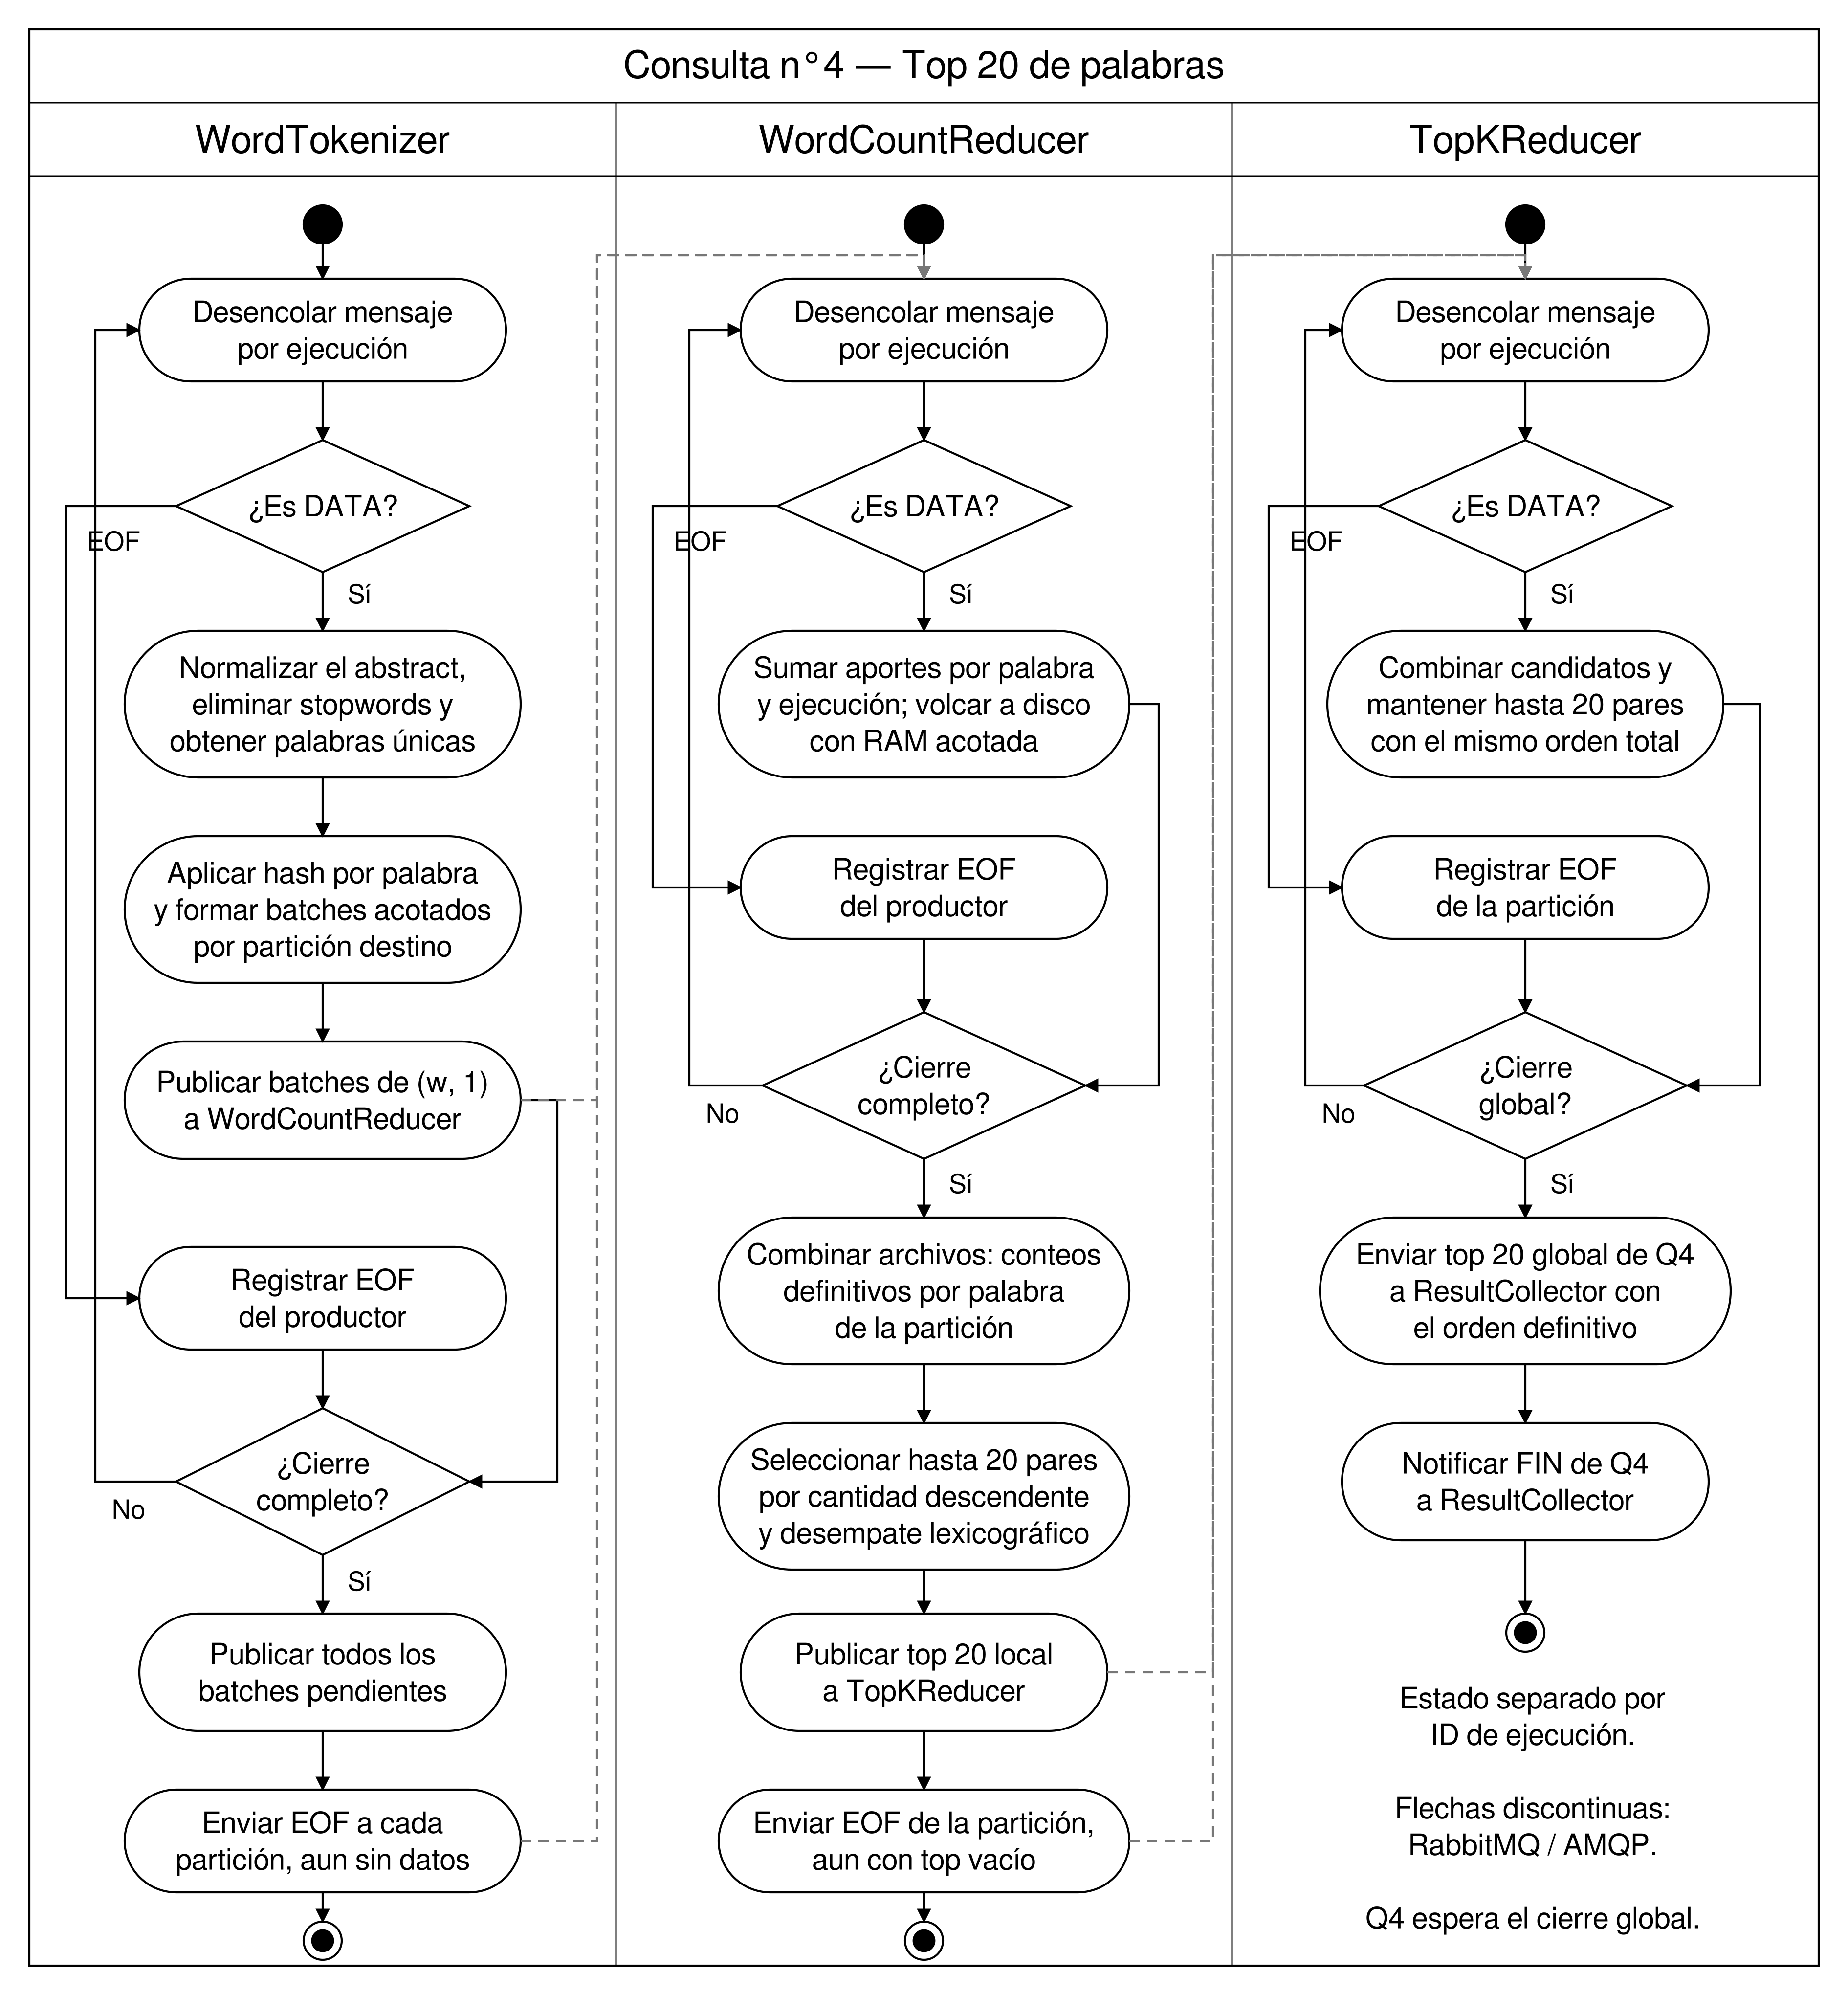
\includegraphics[width=\textwidth,height=0.82\textheight,keepaspectratio]{img/Act/query_4_Act.png}
    \caption{Top 20 de palabras de los abstracts: se excluyen stopwords y cada palabra se cuenta una sola vez por abstract.}
    \label{fig:query-4}
\end{figure}

\subsection{Consulta nº5}

Como ya fue explicado en los diagramas de las queries anteriores, para la query 5 no incluimos el \texttt{WordTokenizer}, a pesar de que este forma parte del flujo de la consulta según lo visto en el DAG. El flujo observado en el diagrama, entonces, comienza en \texttt{WordCounter}, que cuenta las palabras de cada abstract y publica el registro hacia \texttt{DateRouter}.

\texttt{DateRouter} clasifica cada registro según su fecha. Los artículos hasta 2020 inclusive se publican hacia \texttt{AverageCalculator}, porque son los que se necesitarán para calcular el promedio. Los artículos desde 2021 se publican directamente hacia \texttt{AverageFilter}, porque son los candidatos a filtrar. Una vez se confirma que no se recibirán más datos, se notifica del EOF tanto al AverageCalculator como al \texttt{AverageFilter}.

\texttt{AverageCalculator} va guardando los conteos recibidos y una vez se cerciora de que hayan llegado todos, procede a calcular el promedio. Es entonces que publica el promedio obtenido hacia \texttt{AverageFilter}, que acumula los conteos recibidos por \texttt{DateRouter} hasta recibir este dato. A partir de entonces, este último nodo comienza a filtrar cada documento según si la longitud de su abstract supera el promedio o no, para finalmente publicarlos hacia el \texttt{ResultCollector}.


\begin{figure}[H]
    \centering
    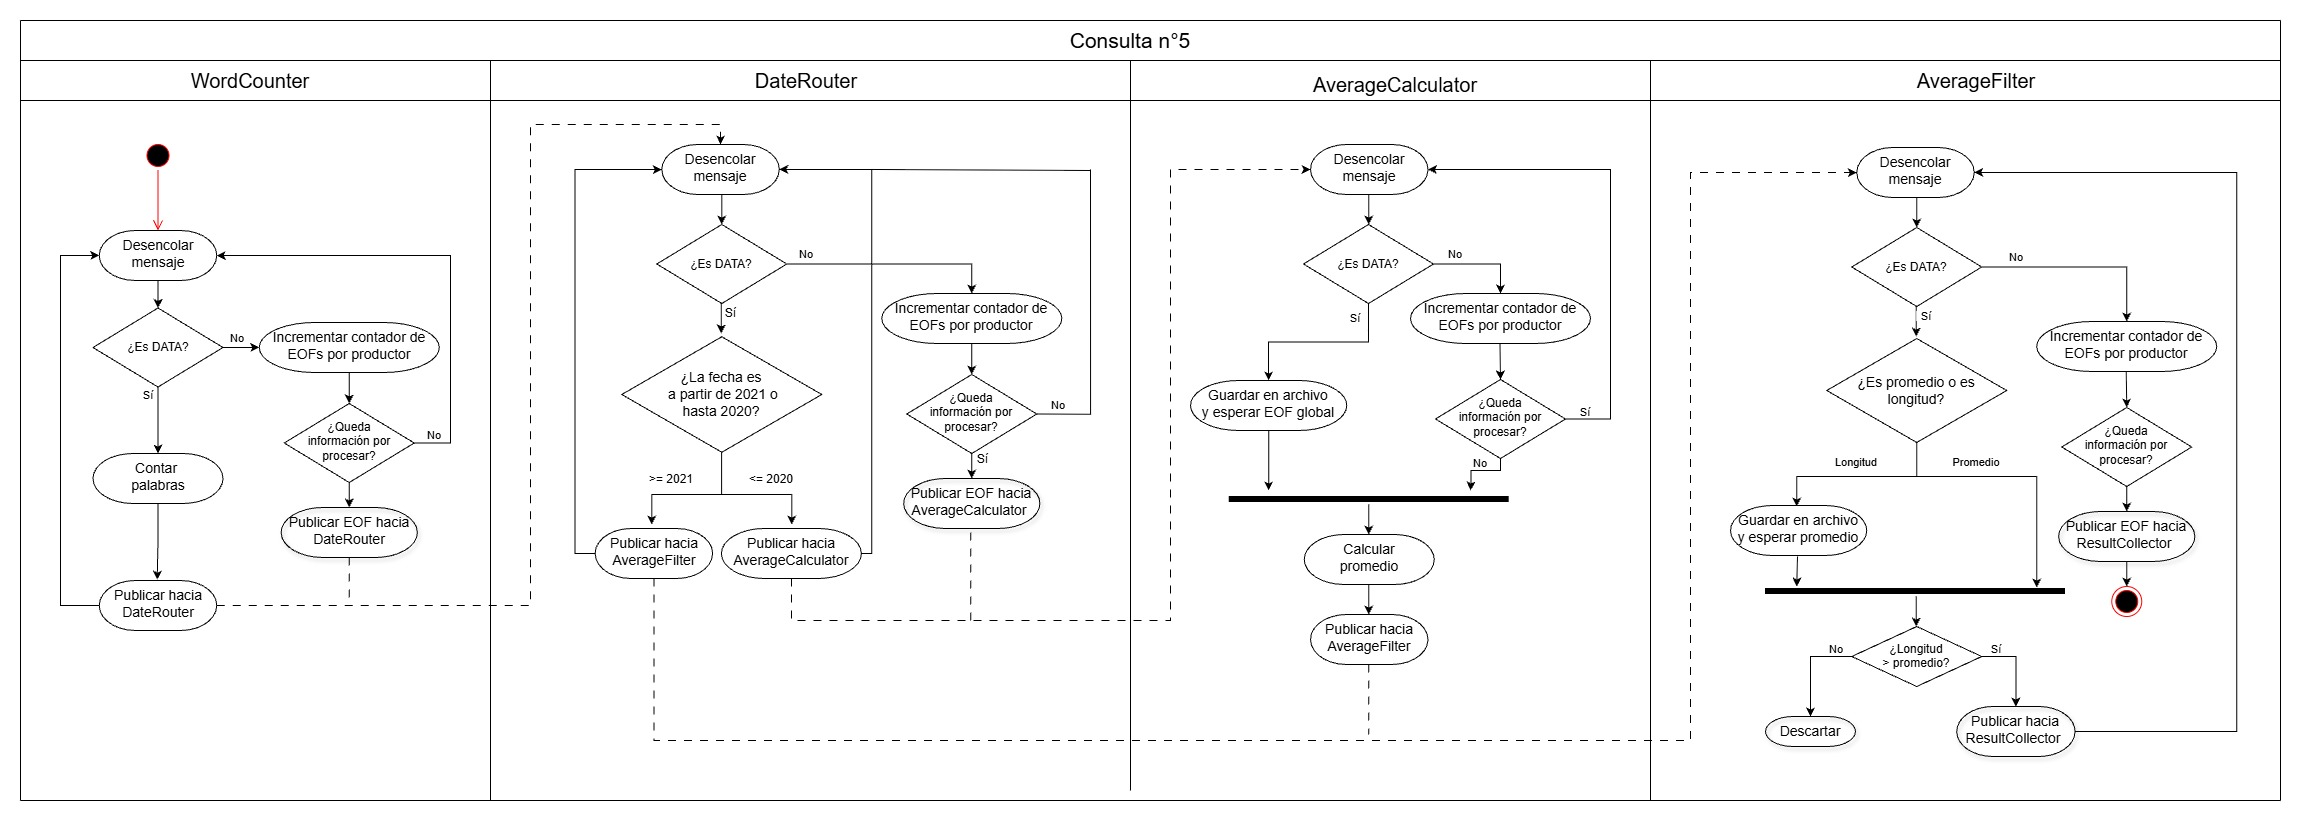
\includegraphics[width=\textwidth,height=0.82\textheight,keepaspectratio]{img/Act/query_5_Act.jpg}
    \caption{Artículos publicados de 2021 en adelante cuyo abstract tiene una longitud superior a la del promedio de los abstracts de los artículos publicados hasta 2020}
    \label{fig:result-collector}
\end{figure}

\subsubsection{Result Collector}
Finalmente, mostramos cómo funcionaría el nodo que comunica al usuario los resultados parciales o totales.
\begin{figure}[H]
    \centering
    \includesvg[width=\textwidth,height=0.82\textheight,keepaspectratio]{img/Act/resullt_collector.drawio}
    \caption{Resolución de primer consulta}
    \label{fig:result-collector}
\end{figure}
\subsection{Diagrama de secuencia}
Para mostrar una idea general de cómo es que los procesos interactuán hicimos un diagrama de secuencia node se muestra todo el flujo del pipeline y el procesamiento en streaming de los Workers de forma abstracta y de los de más nodos de forma explícita.
\begin{figure}[H]
    \centering
    \includesvg[width=\textwidth,height=0.82\textheight,keepaspectratio]{img/diagrama_procesos.drawio}
    \caption{Interacción entre procesos}
    \label{fig:secuencia}
\end{figure}




